
\chapter{Charge Ratio of Atmospheric Muons at IICHEP-Madurai}

As a part of the ICAL R\&D program, a magnetised detector (mini-ICAL)
with 10 layers of RPCs has been built and operational at IICHEP,
Madurai situated near the INO site. Being a scale-down model of the
ICAL detector, the mini-ICAL is being studied a the prototype of
the magnetised ICAL. This prototype is mainly built to study the
performance of electronics equipment in the presence of the magnetic
field and to test the event reconstruction algorithms.
The cosmic ray data collected by the
detector setup is also used to calculate the charge ratio $(R)$
of the number of $\mu+$ to $\mu-$ arriving at the Earth's surface.
The testing of the reconstruction algorithms is the motivation behind
this study. By comparing the result from cosmic ray data with extreme
air shower (EAS) simulation, this study signifies the ability of
the magnet in identifying the charge of the particle.
The cosmic muons are created at the upper atmosphere when high energy
primary cosmic rays interact with the air molecules.
As the primary cosmic rays are dominated by the positively charged
particles, the production of the positively charged mesons are
favoured. The measurement of the muon charge ratio can also be used
to improve the hadronic interaction models and for better neutrino
flux prediction.

\section{Detector Setup of mini-ICAL}
The mini-ICAL detector is consist of 11 layers of iron of size
4\,m\,$\times$\,4\,m\,$\times$\,5.6\,cm with the inter-layer gap
of 4.5\,cm weighing at 85\,Ton. This makes the dimensions of this
prototype detector are 4\,m\,$\times$\,4\,m\,$\times$\,1.06\,m.
The detector setup is shown in the Figure~\ref{fig:miniICAL_iron}
where the $X$-axis of the detector is making an angle of $10^\circ$
with the geographic north.
\begin{figure}[h]
  \centering
  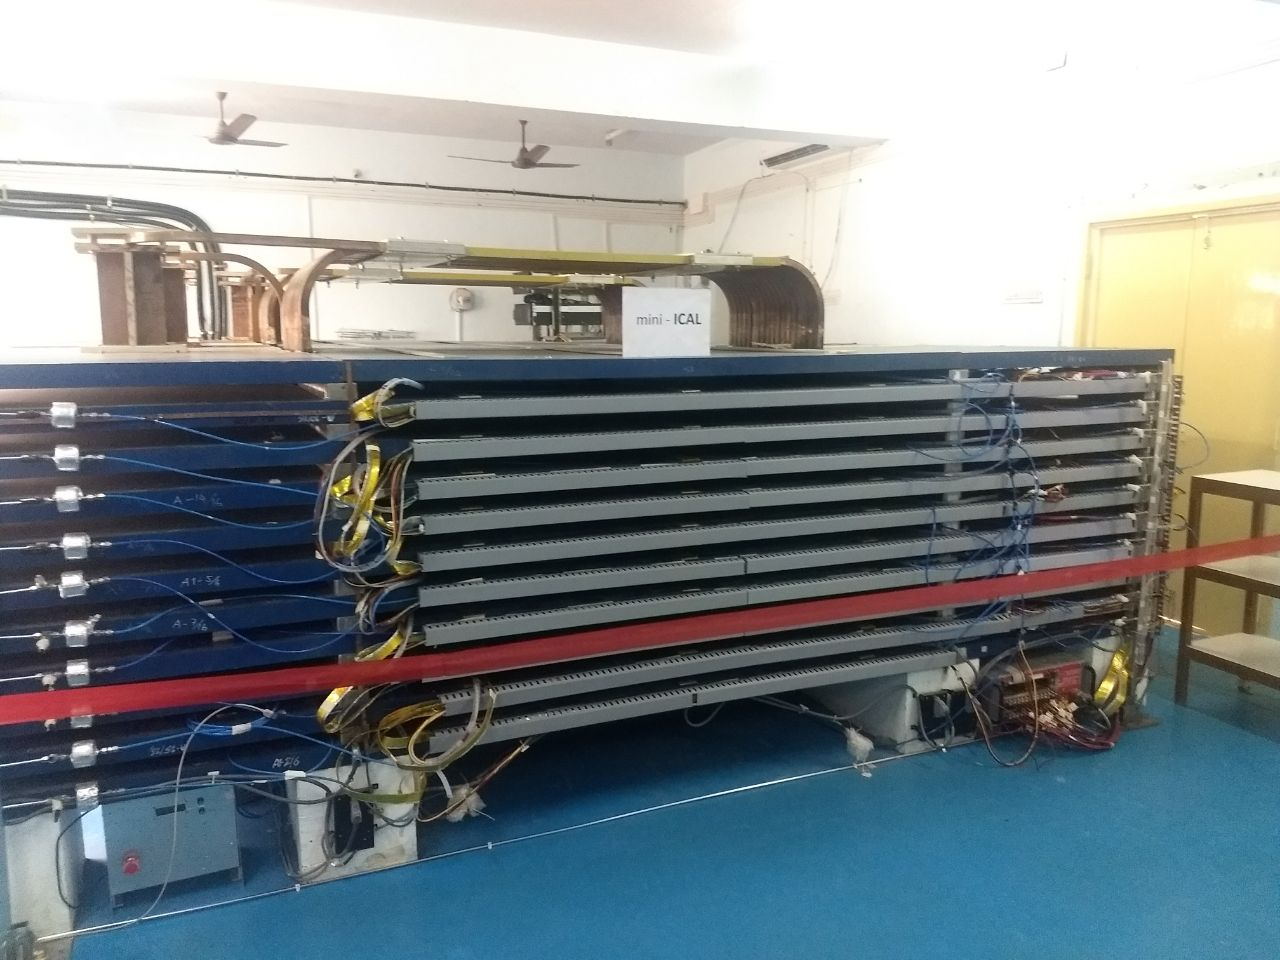
\includegraphics[width=0.49\linewidth]{micalphoto.png} 
  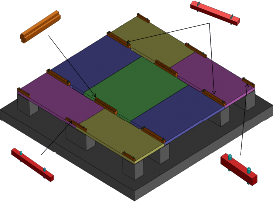
\includegraphics[width=0.49\linewidth]{miniICAL_iron_block.pdf} 
  \caption{(Left) The mini-ICAL Detector Setup (right) and the different
    sections of one layer of iron and the stainless-steel spacers}
  \label{fig:miniICAL_iron}
\end{figure}
The iron layers in the mini-ICAL magnet is made of soft iron with
the additional chemical composition of C\,(0.015\%), Mn\,(0.37\%),
P\,(0.012\%), S\,(0.008\%), Si\,(0.188\%), Al\,(0.001\%), N\,(50\,ppm).
This soft iron has low carbon content which makes it strong enough
mechanically to support its own weight, but also allows it to have high
high permeability with knee point at $\sim$1.5\,T.
Each of the layer of iron is consists of several different tiles shown
in the Figure~\ref{fig:miniICAL_iron}.
The gap between the layers are maintained with the help of the spacers
made of non-magnetic stainless steel (SS-304) shown also in the
Figure~\ref{fig:miniICAL_iron}.

There are four slots with dimensions of 80\,cm\,$\times$\,8\,cm to
accommodate two sets of current conducting coils to create magnetic
field inside the iron in a similar fashion to the proposed
ICAL detector. The coils are made of OFE-grade copper with
oxygen content less than 10\,ppm. There are 18 turns of coils in each
set of coils. Each of the turns are kept at a distance of 40\,mm.
The coils are hollow inside with the cross section of
30\,mm\,$\times$\,30\,mm\,$\times$\,$\phi$17\,mm.
The two sets of coils are electrically connected in series,
and a low voltage power supply is used to supply 900\,Amp
of trough via the coils. An uniform magnetic field of $\sim$1.5\,T
is obtained in the central region of the detector. The magnetic field
in the mini-ICAL is along the (-)Y-direction in the central region.
The heat generated by the current in the
coils are extracted by a closed-loop low conductivity water cooling
system (LCWCS) by flowing chilled water through the bore of the coils.

Ten RPCs of dimensions 174\,cm\,$\times$\,183.5\,cm are used as the
active detector. These RPCs are and placed in the central region of
the detector in between iron layers.
An RPC gap is made of two glass electrodes of thickness 3\,mm with
a gap of 2\,mm between them. Uniform gap between these two electrodes
is maintained using a array of 2\,mm thick poly-carbonate buttons.
The glass gap is sealed on the outer edges to make it air-tight.
A mixture of gases with the compositions of R134a (95.2\%),
iso-C$_4$H$_{10}$ (4.2\%) and SF$_6$ (0.3\%) is flown in the RPCs
via strategically placed nozzles. This mixture of gasses serves as the
target medium of the detector.
Both the outer surfaces of the glass gap are coated with a thin layer
of graphite. The RPCs are operated by applying a differential supply of
$\pm$\,5\,kV to the graphite layers which creates a constant electric
field between the glass electrodes. The ionisation of the gas mixture
by passage of the charged particles eventually evolves into a
avalanche in the presence of the high electric field between the glass
electrodes. The avalanche in the RPCs induces signals in the two
orthogonal pickup panels placed on both sides of the glass gaps
labelled as X-side and Y-side. The pickup panels are made of parallel
copper strips of width 28\,mm with 2\,mm gap between two consecutive
strips. There are 58 strips on the X-side and 61 strips on the
Y-side for each layer.

The DAQ system is similar to the setup discussed in the previous
chapter. In this case the cosmic muon data have been collected using
the 1-Fold signals from top 4 layers as trigger.
An event data typically contains strip hit and timing information
of an event. The strip hit is basically one logic bit per strip
indicating the signal in that strip is above the threshold value
for that strip. The least count of each of the TDC is 0.1\,ns.
The timing data is consists of 16 time signal for
each layer where each multi-hit TDC channel records time signals
coming from every alternating 8$^{th}$ strips on one side of the layer.
The time signal of each hit is recorded for both the leading-edge and
the trailing-edge of the induced signal pulse.


\section{Monte-Carlo Simulation}
The Monte-Carlo Simulation for this study has been executed in
two parts. The Extensive Air Shower (EAS) has been simulated
by the CORSIKA simulation package\cite{corsika763}. The information
of daughter particles generated by the EAS at the earth's surface
level has been extracted and the charge ratio of muons ($R$) is
observed. The $R$ spectra from the CORSIKA prediction is used to
compare the results obtained in the observational data in the
Section~\ref{section:multiresult}.
The detector simulation has been executed with the help
of the GEANT4 toolkit\cite{geant4}. The detector's parameters are
calculated using (efficiency, noise, strip multiplicity and
resolution) are calculated using the cosmic ray data without magnetic
field in the detector. The schemes of the EAS and the
detector simulations are already elaborated in the
Chapter~\ref{chapter:multi}.

Both the events from the observed cosmic ray data and the detector
simulation are reconstructed using the track fit algorithm which is
discussed in the next section.

\section{Event Reconstruction and Data Selection} \label{sec:momreco}
The recorded data is actually the projection of the track on the
\mbox{X--Z} and \mbox{Y--Z} sides. During the passage of a charged
particle through a RPC gap, the number of strips on which signal is
induced depends on the gain of the gas gap. This sharing of the induced
signal between the neighbouring strips is the main reason for the
observed strip multiplicity shown in the Figure~\ref{fig:layer2y}(c).
In order to prepare the events for analysis, the consecutive strips
which have recorded signal are clubbed together to form a cluster.
The layers with no clusters either or both on X and Y sides are
neglected during the track reconstruction.

During the study, the position resolution for strip multiplicities of
1, 2 are $\sim$6\,mm. In this study, the clusters of hits with more
than 2 multiplicities are neglected as the position resolution for
higher multiplicities is found to be the worse. A layer which has
more than 15 strip hits and/or more than 10 clusters is tagged as
`noisy layer' and not considered in the track reconstruction. An
event which has more than 3 noisy layers is considered as
`noisy event' and discarded.

Now, as it shown earlier, the strength of magnetic field in the
X-direction is very small. So, almost no significant bending is
observed in the Y-side of the track which makes the projection of
the track on the Y-side to be fit with a straight line.
Thus, in the first step of track reconstruction, the clusters on
the Y-side associated with the tracks are found and grouped using
the method of Hough Transformation\cite{hought}. This eliminates
the possibility of noise hits on the Y-side getting included in the
track reconstruction. Once one valid straight track found, attention
is given on the X-side of the track. As the magnetic field is mainly
in the Y-direction, maximum bending of track is observed on the X-side.
The clusters on the X-side is then fitted with a circle.
The information of the fitted circle helps to reject the noise hits
on the X-side as well.
Using the radius ($r$ in meter) of the fitted circle, the transverse
momentum ($p_t$ in GeV) of the particle can be roughly estimated by
the following equation,
\begin{equation}
  p_{t}=0.3Br \label{eq:pt_est}
\end{equation}
where, $B$ is the average magnetic field in Tesla.
The information of the fitted straight line on Y-side and the circle
on the X-side further used to calculate the direction (zenith and
azimuth) and the location of incidence of the particle roughly.

The momentum vector and the location of incidence, estimated
above are given as the input parameter to the track reconstruction.

The particle is propagated in the medium of the detector by integrating
the following equation numerically,
\begin{equation}
  \vec{\ddot{x}} = \left(\frac{q}{\gamma m_{\mu}}\right)\vec{\dot{x}}\times \vec{B}
\end{equation}
where, $\vec{\dot{x}}=\frac{\vec{p}}{\gamma m_{\mu}}$ and
$\gamma=\sqrt{1+\left(\frac{p}{m_{\mu}c}\right)^{2}}$.

A time-step of 10\,ps is used to propagate the particle in the
detector. This is equivalent to a step-size of $\sim$3\,mm at speed
of light. At each step of the propagation the ionisation energy
loss of the particle is calculated using the graph shown in
the Figure~\ref{fig:eloss}.
%% will add this plot later

The 5 parameters (3 momentum parameters and 2 position parameters) are
properly estimated by minimising the least-squared distance
($\chi^{2}$/ndf).
The exhaustive grid-search method have been adopted to minimised the
$\chi^{2}$ as the maximum number of data points available is only 10.
Any other methods are are avoided as the chances of minimising the
$\chi^{2}$/ndf to a local minima is very high with smaller number of
data points.

A few events with reconstructed track are displayed in the
Figure~\ref{fig:eventdisplay}.
\begin{figure}[h]
  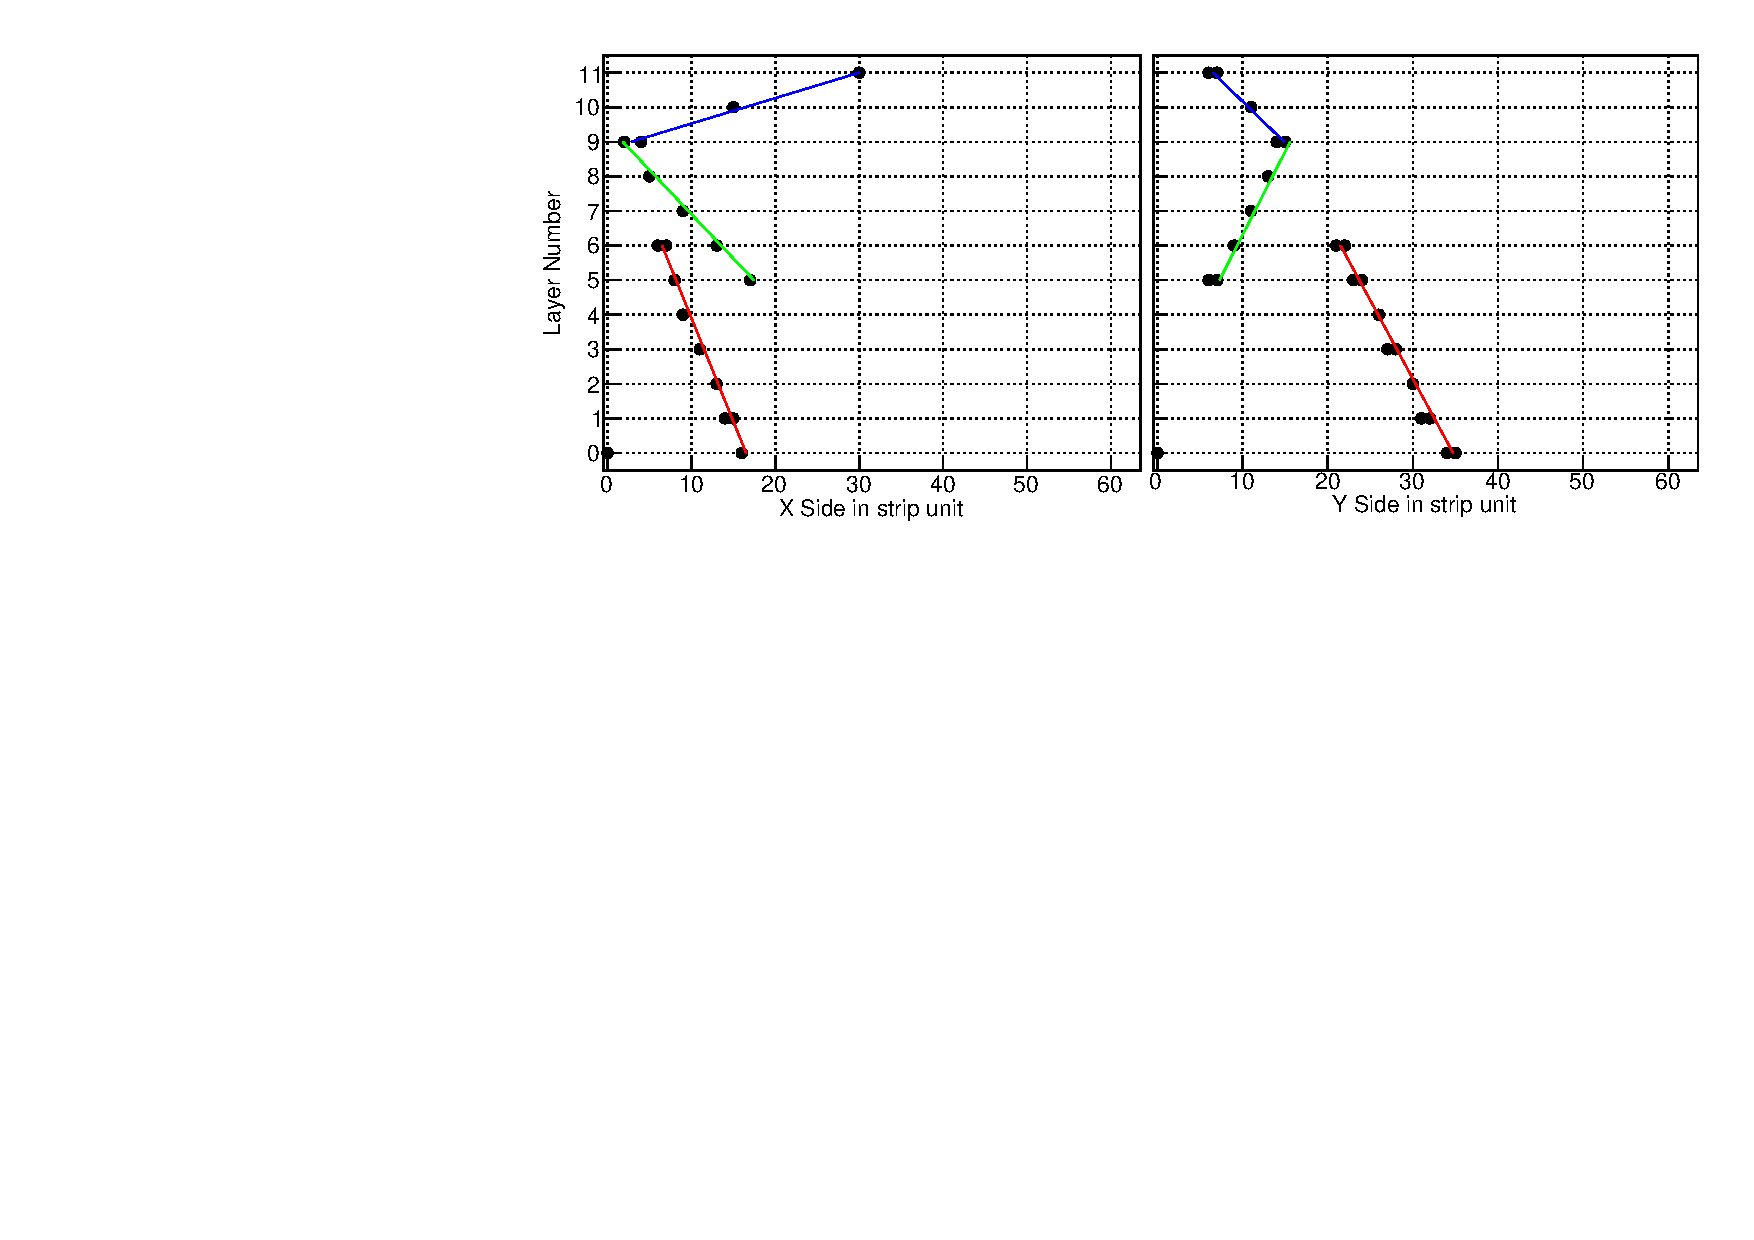
\includegraphics[width=1.0\linewidth]{Multi_Event_20170823_102605_361367_Inside_1.pdf}
  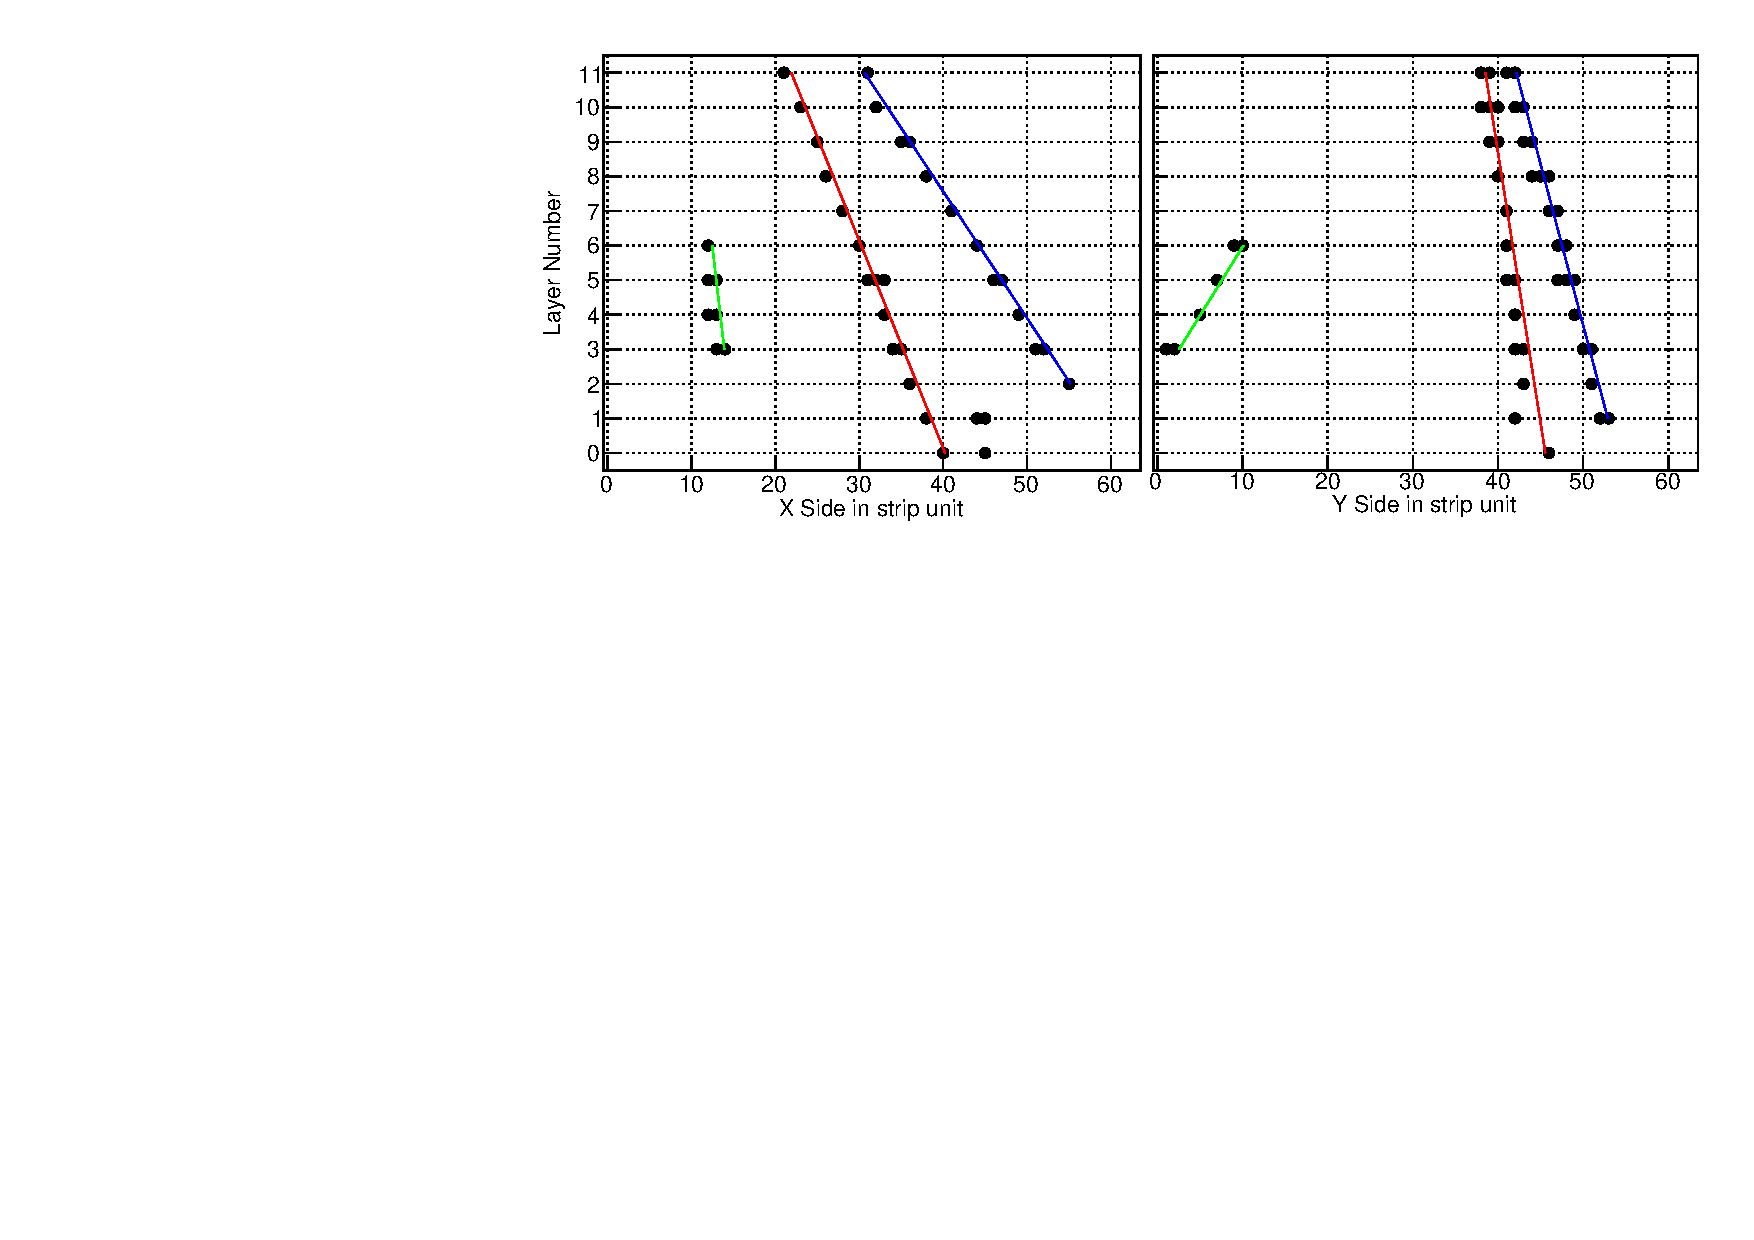
\includegraphics[width=1.0\linewidth]{Multi_Event_20170823_102605_9676_Roof_1.pdf}
  \caption{Two events with reconstructed track. (To be replaced later)}
  \label{fig:eventdisplay}
\end{figure}
A track is considered as properly reconstructed if the $\chi^{2}$/ndf
is less than 5 (in strip unit) and there are more than 7 layers in
the track.

\section{Charge Ratio Spectra of Cosmic Ray Muons}
\label{section:multiresult}
The measured momentum spectra in the reconstruction process is biased
because of the housing building covering the detector, limited
acceptance of the detector, resolution and other systematic effects
on the detector. So, to compare the experimental measurement with the
CORSIKA prediction, the reconstructed spectra is unfolded to eliminate
the detector's effects.
The unfolding method used for the current study is iterative
Bayesian Unfolding \cite{bayesian}.
The response matrix derived from the MC simulated events in the
GEANT4 using the reconstruction method described in the
Section~\ref{sec:momreco} is shown in the
Figure~\ref{fig:unfolddata}(a).
\begin{figure}[h]
  \includegraphics[width=1.0\linewidth]{unfoldedmom.pdf}
  \caption{(a) The Response Matrix, (b) Unfolded Momentum Spectra for
    $\mu^{+}$ and $\mu^{-}$ reconstructed from data, (c) Charge Ratio
    of muons.}
  \label{fig:unfolddata}
\end{figure}
To eliminate any bias in the response matrix between $\mu^{+}$ and
$\mu^{-}$, equal numbers of $\mu^{+}$ and $\mu^{-}$ are simulated in
the GEANT4 with the azimuth ($\phi$) generated uniformly, the zenith
($\theta$) generated using $\sin^{2} \theta$ spectra and the energy
($E$) using $E^{-2.7}$ spectra in the MC simulation.
In the Bayesian technique, the background in each reconstructed
momentum bin and efficiency of each true momentum bin are calculated.
The reconstructed data and MC are also corrected for fake rate.

The unfolded momentum spectra for muon is shown in the
Figure~\ref{fig:unfolddata}(b). The charge ratio spectra of cosmic
muons reconstructed from observational data and CORSIKA prediction
are shown in the Figure~\ref{fig:unfolddata}(c). It can be seen that
the ratio between $\mu^{+}$ and $\mu^{-}$ matches up to the energy
of $\sim$12\,GeV.

\section{Chapter Summary}
As a part of the ICAL R\&D program, a magnetised detector
(named mini-ICAL) with 10 layers of RPCs interspersed with 56\,mm iron
layers has been built and operational at IICHEP, Madurai situated
near the INO site. The cosmic ray data collected by the detector
setup is used to calculate the charge ratio $(R)$ of the number
of $\mu+$ to $\mu-$ arriving at the Earth's surface.
Using the iterative Bayesian Unfolding technique, the charge ratio
of muons is observed and compared with the CORSIKA prediction.
From the study, it is seen that the ratio between $\mu^{+}$ and
$\mu^{-}$ more or less matches in the range of 1-6\,GeV.
The reconstruction of momentum beyond this energy fails due to the
insignificant curvature of the tracks created by the particles, poor
position resolution of RPCs, limited number of tracker layers and
the energy cutoff in this detector setup.
